\chapter{Implementazione} \label{implementazione}
Avendo già definito il contesto in cui il \textit{WarehouseBackendWorker} andrà ad inserirsi, il lavoro che esso andrà a svolgere ed un primo abbozzo alle ottimizzazioni, una grande parte del lavoro può dirsi completata. Tuttavia, in fase di implementazione, sorgono molti problemi e conseguenti soluzioni, dovendo mettere in pratica ciò che si era trattato solo ad alto livello; è quindi necessario ragionare circa eventuali \textit{trade off}, approssimazioni eventuali, e, ovviamente, fare i conti con le limitazioni ed i punti di forza delle tecnologie che si stanno impiegando. In questo capitolo si introduce innanzitutto il linguaggio con cui il worker è stato realizzato, successivamente si mostrano le fasi di sviluppo del software che ne dà la vita, e, infine, si trattano alcune delle ottimizzazioni discusse precedentemente.
\section{Il linguaggio: Go}
Go \cite{go} (anche denominato \textit{Golang}) è un linguaggio Open Source compilato e staticamente tipizzato, pensato appositamente per essere semplice nella sintassi. Essa risulta difatti molto simile a quella del linguaggio C, mossa strutturale pensata appositamente per non rendere il passaggio tra un linguaggio ed un altro arduo. 
\begin{wrapfigure}{r}{0.25\textwidth}
\centering
    
\includegraphics{images/gopher.png}
    \caption{Gopher, la mascot di Go.}
    \label{fig:gopher}
\end{wrapfigure}
Go supporta l'uso di un \textit{Garbage Collector} (\textit{GC}) che ottimizza automaticamente l'uso della memoria, l'uso delle \textit{Reflection} per conoscere, ad esempio, il tipo delle variabili a run-time, e fornisce un meccanismo built-in per la concorrenza sotto forma di una metodologia a scambio di messaggi all'interno dei \textit{Canali}. Uno dei punti di forza, esterni alle caratteristiche intrinseche del linguaggio, risiede nella forza della comunità di sviluppatori che contribuiscono al miglioramento di Go; un esempio calzante dello spirito di comunità è chiaro se si pensa che il linguaggio ha addirittura una mascot (creata da Renee French), mostrata in Figura \ref{fig:gopher}. Proprio grazie a questo forte senso di comunità, la ridistribuzione del codice sorgente online per progetti, utilità e strumenti è particolarmente favorita. Per rendere disponibile il proprio codice ad altri sviluppatori, è fondamentale il concetto di \textbf{Moduli} e \textbf{Package}. In Go, un Modulo è un insieme di package, ed è propriamente l'elemento che uno sviluppatore può pubblicare e condividere. Un Package, invece, è un insieme di codice sorgente. Eventualmente, un Package può contenere altri Package.

\paragraph{Go in SeismoCloud} 
Nel progetto SeismoCloud, Go è utilizzato principalmente per la realizzazione delle API esposte all'utente, per alcuni worker che eseguono compiti specifici periodici (prendendo un esempio, la chiusura di una chat, lavoro dello studente Emanuele Petriglia \cite{emanuelepetriglia}) e per il \textit{WarehouseBackendWorker}, oltre ad altro codice sorgente di utilità per il lavoro.
In particolare, nell'ambito del Back End dell'applicazione SeismoCloud, il codice è contenuto all'interno di una repository e rappresentato da un modulo, con all'interno due package che svolgono compiti ben precisi: il package \textbf{cmd}, che contiene una serie di package rappresentanti i codici eseguibili, ed il package \textbf{service}, che rappresenta un singolo servizio per ogni package al suo interno. Contestualizzando quanto detto, in Figura \ref{fig:seismopackage} sono mostrati i package presentati.
\begin{figure}[h!]
    \centering
    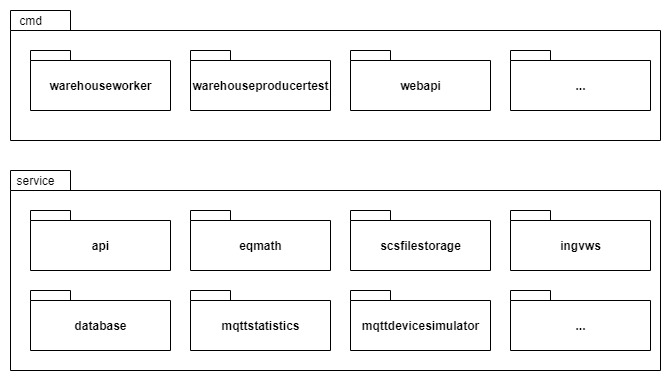
\includegraphics[width=\textwidth]{images/seismopackage.jpg}
    \caption{I package in SeismoCloud.}
    \label{fig:seismopackage}
\end{figure}
Uno dei package contenuto in \textbf{cmd}, e sviluppato per la realizzazione del codice eseguibile del \textit{WarehouseBackendWorker}, è \textbf{warehouseworker}: esso permette di rendere operativo il worker quando viene eseguito il codice. Invece, per citare un package in \textbf{service}, \textbf{eqmath} è un package che fornisce funzioni utili per alcuni calcoli relativi alla geometria spaziale, come il determinare se un punto (individuato da latitudine e longitudine) si trova all'interno di una data area geografica.\footnote{Questa funzione, nello specifico, è stata utilizzata nel corso dell'implementazione, per questo motivo è stata selezionata come esempio in questa sezione relativa alla correlazione tra Go e SeismoCloud.}

\section{Il WarehouseBackendWorker}
%definizione della struct Query e relativo code snippet
Nella sezione \ref{messageformat} si è mostrato il formato concordato per permettere una comunicazione unitaria tra Producer e Consumer di NSQ. Ovviamente, per poter essere utilizzato, il messaggio necessita di una mappatura 1-to-1 nei suoi campi con un elemento del linguaggio Go; un modo immediato di farlo è definire un \textbf{type} per la richiesta stessa, funzionalità permessa dal linguaggio di programmazione in questione. Il tipo scelto prende il nome di \textbf{Query} ed è una struct composta da tutti gli elementi definiti ed inseriti nel messaggio, per l'appunto. Il Codice Sorgente \ref{code:messageimpl} vuole essere sia un primo esempio dimostrativo di codice in Go, sia rappresentare il tipo Query stesso. 
\begin{listing}[h!]
\inputminted[baselinestretch=0.8]{go}{sources/query.go}
\caption{Il tipo Query.}
\label{code:messageimpl}
\end{listing}
Concentrandosi sul codice, si può notare come molti elementi siano di un tipo predefinito: \textbf{string}. Altri, come \textbf{Attributes}, sono tipi creati appositamente. I campi della struct Query non richiedono una spiegazione approfondita: essi rappresentano la loro controparte nel formato del messaggio, di cui si è già discusso in precedenza\footnote{Una nota importante, che permette di comprendere come lavori internamente il json decoder: il codice che presenta il pattern `json:"something"` è una caratteristica peculiare di Go, chiamata \textit{tag}. Con il tag, è possibile semplificare il lavoro del decoder indicandogli a quale chiave corrisponde nel JSON il campo in questione.}.

\paragraph{Il Consumer}
Creata una struttura per la rappresentazione del messaggio in Go, è ora necessario creare il Consumer. Propriamente, la creazione del consumer risulta abbastanza intuitiva, dovendogli solamente fornire (rimembrando il funzionamento di NSQ descritto in \ref{warehousedesign}) il nome del topic e del channel da cui riceverà i messaggi, oltre che un parametro di configurazione di NSQ. Bisogna poi registrare un \textit{Handler} che effettivamente svolga delle operazioni sul messaggio: senza alcun \textit{Handler}, il messaggio viene soltanto recapitato al Consumer, che non fa nulla. L'\textit{Handler} da registrare non è altro che un'interfaccia, denominata, per l'appunto, \textbf{Handler}. Questa interfaccia ha un solo metodo, la cui firma è:
\begin{minted}{go}
func HandleMessage(message *nsq.Message) error
\end{minted}
In Go, il concetto di interfaccia e di tipo che la implementa è abbastanza sottile: un tipo implementa implicitamente una interfaccia se esso implementa ogni metodo dell'interfaccia stessa. Per cui, per poter implementare l'interfaccia \textbf{Handler} e registrare un \textit{Handler} per la lavorazione dei messaggi, basta che una struttura implementi il metodo mostrato sopra. La struttura creata che lo implementa è il \textit{warehouseBackendWorker}, mostrata nel Codice Sorgente \ref{code:warehousebackendworker}.\footnote{In realtà, la situazione è leggermente più intricata, in quanto come Handler è registrata un'interfaccia ulteriore, che il warehouseBackendWorker implementa a sua volta. Questa situazione nasce da un discorso di visibilità dei tipi e per un corretto uso di alcune code practise, ma, ai fini di quanto trattato, è ininfluente.}
Si vuole far notare che, prima di raggiungere le versioni del codice presentato in tutto il capitolo, sono state necessarie diverse iterazioni che studiassero ed implementassero soluzioni sempre migliori. Questi raffinamenti possono essere approssimativamente inquadrati in tre fasi: 
\begin{itemize}
    \item Implementazione delle funzionalità principali.
    \item Implementazione della Streaming Pipe.
    \item Implementazione del Contesto della richiesta.
\end{itemize}
Lo scopo del capitolo non è confrontare in modo verboso i singoli cambiamenti tra le versioni, ma di dare un'idea del ragionamento alla base di essi e del perché sono stati introdotti. Per tale motivo verrà mostrato solamente il codice dell'ultima versione, e non i codici intermedi, ma se ne discuterà per evidenziarne le criticità, risolte poi dai suddetti cambiamenti. 

\begin{listing}
\inputminted[baselinestretch=0.8]{go}{sources/warehousebackendworker.go}
\caption{Il tipo warehouseBackendWorker.}
\label{code:warehousebackendworker}
\end{listing}

\section{Implementazione delle funzionalità}
I messaggi che vengono recapitati al Consumer sono elaborati dal worker, e, in particolare, dalla funzione \textit{HandleMessage}, riportata nel Codice Sorgente \ref{code:handlemessage}.
\begin{listing}
\inputminted[baselinestretch=0.9]{go}{sources/handlemessage.go}
\caption{La funzione che processa le richieste.}
\label{code:handlemessage}
\end{listing}
In esso sono trascurati alcuni elementi che coinvolgono i messaggi inseriti nel log e gli errori ritornati, tranne per la loro prima occorrenza: si vuole difatti evidenziare come il ruolo giocato dal log sia fondamentale per risalire ad eventuali errori o problemi nel corso del ciclo di vita del software e come il linguaggio consideri gli errori; essi sono gestiti esplicitamente, ed è buona pratica che una funzione abbia come tipo di ritorno un errore (che è un tipo built-in). La funzione è di per sé molto semplice: essa, difatti, demanda ogni compito del worker ad altre funzioni (si vedano \textit{GetResultsFromLocation} e \textit{SendNotification}). L'idea alla base è di identificare ogni compito delineato nella Figura \ref{fig:workerflow} con una funzione, in modo da modularizzare, ove possibile, il codice, rendendolo semplice, intuitivo e manutenibile, e rispettando sia i canoni dell'Ingegneria del Software, sia lo stile organizzativo del progetto. Una prima eccezione è l'estrazione e la consegna del messaggio, che vengono effettuate "automaticamente" secondo il meccanismo definito dal package NSQ, per cui non ha necessità di una funzione dedicata, così come la decodifica del messaggio, servizio offerto dalla libreria \textit{encoding/json}, e, in particolare, dalla funzione \textbf{json.Unmarshal}. 
\\
\\
Seguendo la pipeline delle istruzioni del worker, le funzioni \textit{GetResultsFromLocation} e \textit{GetResultsFromDevices} gestiscono le interrogazioni del Database, la scrittura dei file ed il caricamento su MinIO.\footnote{La dicitura "Location" al termine delle funzioni sviluppate sta ad indicare il soddisfacimento delle richieste che richiedono i dati non tramite Sismometri, ma tramite un'area geografica. Lo stesso discorso vale per "Devices". Questa distinzione è necessaria per alcune operazioni aggiuntive che devono essere effettuate nelle richieste con la dicitura Location, oltre che per favorire, ancora una volta, la semplicità e la modularità del codice. A livello pratico potrebbero essere accorpate nelle altre funzioni, ma minerebbero di molto questo stile di scrivere codice organizzato.} Prendendo come esempio \textit{GetResultsFromDevices} (Codice Sorgente \ref{code:getresults}), i passi che essa esegue per ogni attributo (ignorando la più volte chiamata \textit{CheckContextStatus}, di cui si parla in \ref{contesto}), in base agli attributi richiesti, sono:
\begin{enumerate}
    \item Chiamare una funzione Get\textit{Attributo}Query.
    \item Chiamare una funzione UploadQueryResultsByDevices.
\end{enumerate}
\begin{listing}[h!]
\inputminted[baselinestretch=0.8]{go}{sources/getresults.go}
\caption{La funzione che gestisce interrogazioni ed upload.}
\label{code:getresults}
\end{listing}
La prima effettua una query al Database relativa all'attributo di cui porta il nome, come \textbf{GetTemperatureQuery}. La seconda è una funzione che si occupa di effettuare la scrittura dei file e l'upload implicito su MinIO, dividendo i compiti in altre funzioni che scrivono ognuna un formato diverso di file (la funzione \textit{UploadCSVByLocation} si occupa dei file CSV ad esempio). Le funzioni che effettuano le query devono essere funzioni che assolvono solamente a tale scopo, per rispettare lo stile delle funzioni simili nel progetto.\\ \\
Le interrogazioni sono piuttosto semplici, per cui non ne verrà mostrato un esempio; è invece necessario concentrarsi su una qualsiasi delle funzioni per la scrittura dei file, come la già nominata \textit{UploadCSVByLocation}, riportata in breve nel Codice Sorgente \ref{code:uploadcsv}. L'aspetto saliente da notare ora è la \textbf{scrittura} del file all'interno del ciclo \textit{for}: si itera finché è presente un ulteriore risultato; ad ogni iterazione:
\begin{enumerate}
    \item Si inseriscono i dati della riga corrente di \textit{rows} in una struttura dati creata appositamente per contenerli.
    \item Si verifica che la posizione del sensore sia all'interno del raggio dell'area specificata nella richiesta. Si utilizza a tal proposito una funzione del package \textbf{eqmath} di SeismoCloud, ma i dettagli sono poco rilevanti in questo discorso.
    \item Il \textit{csvWriter}, una variabile di tipo puntatore a csv.Writer, scrive le informazioni presenti in \textit{csvLine} all'interno di \textit{fileInZipCSV}, un puntatore ad un file contenuto nell'archivio ZIP che si ottiene al termine del lavoro.
\end{enumerate}
Il meccanismo pensato specificamente per l'upload è discusso in \ref{streamingpipe}, dove apparirà chiaro il ruolo della variabile \textit{fileInZipCSV}.
\begin{listing}[h!]
\inputminted[baselinestretch=0.8]{go}{sources/uploadcsv.go}
\caption{La funzione che effettua la scrittura dei file e l'upload.}
\label{code:uploadcsv}
\end{listing}
Avanzando temporaneamente su questo aspetto, l'ultimo compito del worker riguarda il notificare l'utente che la richiesta è stata elaborata. Come già accennato, \textit{SendNotification} è la funzione preposta a fare ciò: essa chiama al suo interno funzioni diverse in base al metodo di invio della notifica scelto dall'utente. Una peculiarità delle funzioni di notifica implementate è che, nella gestione degli errori, qualsiasi errore è sempre inserito nel log ed ignorato, in quanto il lavoro è stato ultimato e non necessità di un'interruzione del flusso di esecuzione dei compiti. La notifica è una funzionalità extra offerta all'utente, che può comunque controllare lo status della propria richiesta tramite le API. La funzione è mostrata nel Codice Sorgente \ref{code:sendnotification}.
\begin{listing}[h!]
\inputminted[baselinestretch=0.8]{go}{sources/sendnotification.go}
\caption{La funzione che si occupa di inviare le notifiche.}
\label{code:sendnotification}
\end{listing}

\section{Implementazione della Streaming Pipe} \label{streamingpipe}
Nella precedente sezione si è mostrata la struttura ed il funzionamento generale del worker, posponendo però un passo importante: l'upload effettivo su MinIO. Inizialmente, esso era stato pensato in modo semplice, schematizzato nella Figura \ref{fig:salvataggiolocale}. Il problema che si sarebbe presentato una volta messo in funzione il sistema avrebbe però riguardato i file, che, esaudita una richiesta, sarebbero rimasti nello storage del server finché un'entità (fisica o digitale) non li avesse rimossi. Progettare un ulteriore worker che ripulisse lo spazio da file obsoleti non sembrava una via praticabile, tantomeno la migliore.
\begin{figure}[h!]
    \centering
    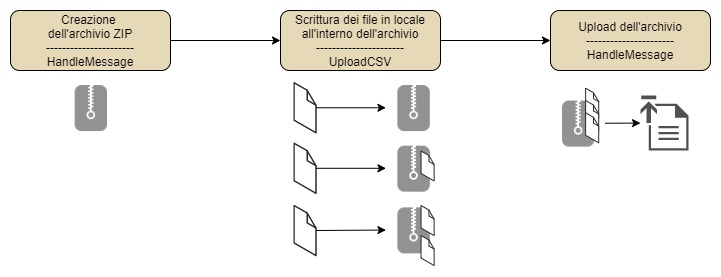
\includegraphics[width=\textwidth]{images/salvataggiolocale.jpg}
    \caption{Upload dei risultati con salvataggio locale}
    \label{fig:salvataggiolocale}
\end{figure}
Una versione aggiornata prevedeva la creazione di file temporanei, di cui il sistema operativo avrebbe gestito autonomamente l'eliminazione. Sembra una soluzione altamente più accettabile, ma le problematiche che continuano a presentarsi sono due: 
\begin{itemize}
    \item Il worker deve comunque scrivere sul disco, che si traduce in spendere maggiore tempo per ogni richiesta (si pensi, in caso di HDD, al tempo di accesso al disco, di rotazione, di ricerca, ecc.).
    \item Il worker esegue i propri compiti linearmente: crea innanzitutto l'archivio ZIP; finché non termina la scrittura di ciascuno dei file, il file ZIP non viene chiuso (allegando un file che funge da una sorta di indice con informazioni sui file presenti al suo interno). Per cui, i compiti sono eseguiti in ordine, con ogni step che deve attendere quello precedente per essere iniziato. In altre parole, l'upload deve attendere finché l'ultima riga dell'ultimo file è scritta. 
\end{itemize}
Si è pensato ad una soluzione che riuscisse a risolvere entrambe le problematiche. In particolare, per evitare l'accesso al disco si potrebbe pensare di memorizzare ogni dato scritto in memoria RAM; il problema evidente è la pericolosità di mantenere tutti i dati scritti in memoria, considerando la mole che ne deriverebbe da ogni richiesta: sebbene sia possibile aggregare e configurare memorie per estenderne la capacità totale, è sbagliato cercare un'ottimizzazione che sembra aggirare il problema invece che risolverlo, basandosi essa solamente sull'aumentare la memoria a disposizione. Se, tuttavia, i dati fossero scritti in modo progressivo mentre sono consumati altrettanto progressivamente, la memoria principale non si troverebbe sommersa di tutta la quantità dei dati scritti, ma di volta in volta di una certa frazione di essi. Dovrebbe essere creato un buffer che gestisce in automatico la sua dimensione, accettando dati in ingresso (la scrittura dell'archivio ZIP) e svuotandosi (upload su MinIO di porzioni dell'archivio) automaticamente. Il buffer non necessiterebbe di scrivere sul disco, ma rimarrebbe in memoria senza sovraccaricarla. L'idea è rappresentata in Figura \ref{fig:pipe}. 
\begin{figure}[h!]
    \centering
    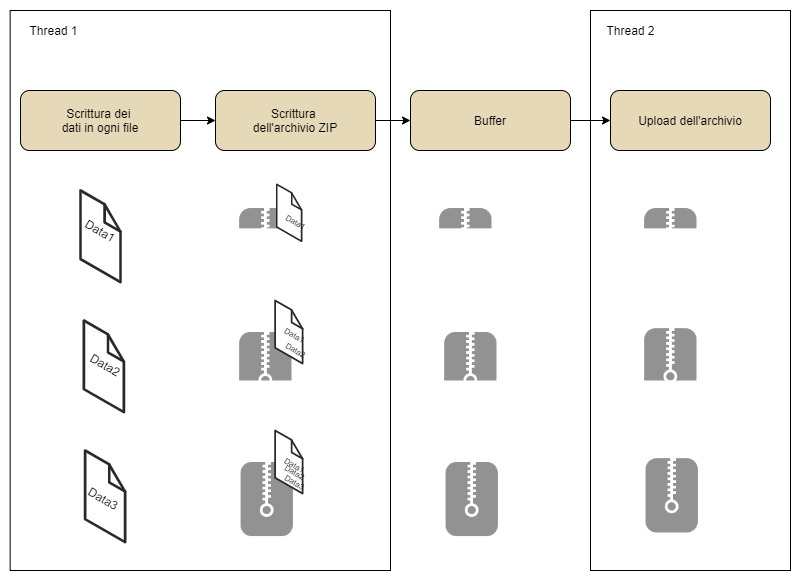
\includegraphics[width=\textwidth]{images/pipe.jpg}
    \caption{Sistema asincrono in memoria per la scrittura e l'upload.}
    \label{fig:pipe}
\end{figure}\\
Dal punto di vista implementativo, una funzione che il linguaggio Go mette a disposizione è \textbf{Pipe()}, del package \textit{io}. Essa crea una pipe in memoria, di cui permette la gestione in scrittura e lettura con i rispettivi valori di ritorno: \textit{PipeWriter} e \textit{PipeReader}. Le due estremità della pipe sono collegate direttamente; non esiste un buffering interno tra loro. Come si può vedere nel Codice Sorgente \ref{code:getresults}, la pipe è creata con l'istruzione:
\begin{minted}{go}
pipeReader,pipeWriter := io.Pipe()
\end{minted}
L'estremità di scrittura pipeWriter è collegata con \textit{writer}, uno zip.Writer che si occupa di scrivere l'archivio ZIP, tramite l'istruzione 
\begin{minted}{go}
writer := zip.NewWriter(pipeWriter)
\end{minted}
Questo comando specifica che l'archivio deve essere scritto \textbf{direttamente} all'interno della pipe, non toccando il disco.
Qualche riga di codice più avanti, invece, si delega ad una goroutine\footnote{Una goroutine è un thread gestito direttamente da Go che viene eseguito in parallelo rispetto al thread principale} l'upload su MinIO, collegando il lato reader della pipe all'interno della funzione preposta al caricamento:
\begin{minted}{go}
worker.fs.PutWarehouseResults(..., pipeReader, ...)
\end{minted}
Questa funzione effettua una serie di HTTP PUT verso il sistema di storage, elemento fondamentale per permettere un caricamento progressivo dei dati su di esso.
La variabile \textit{writer} viene poi passata in input a \textit{UploadQueryResultsByDevices}, che si collega alla funzione:
\begin{minted}{go}
func UploadCSVByLocation(userRequest Query,rows pgx.Rows,
zipWriter*zip.Writer,fileNamestring) error
\end{minted}
mostrata nel Codice Sorgente \ref{code:uploadcsv}. Si era detto che l'utilità della variabile \textit{fileInZipCSV} sarebbe stata chiarificata successivamente: ebbene, essa rappresenta un file che lo zip.Writer, creato in precedenza e passato in input, origina. In questo modo, i dati scritti ad ogni iterazione del ciclo \textit{for rows.Next()} sono inviati lungo questa catena di writer, fino a giungere alla goroutine, che continuerà a ricevere i dati di volta in volta, effettuando un upload progressivo. Questo sistema è stato chiamato \textit{Streaming Pipe}.

\section{Implementazione del Contesto} \label{contesto}
Allo stato descritto fin'ora, il sistema, in casi eccezionali, potrebbe andare in stallo e non terminare su una data richiesta; il rischio è che, per qualche problema, esso continui ad eseguire operazioni pesanti dal punto di vista dell'intero sistema, come la scrittura o il caricamento dei file. Un comportamento del genere non gestito, ovvero terminato, porterebbe ad un possibile collasso del server su cui il codice è installato. Qui entra in gioco il \textbf{Contesto} di una richiesta: le richieste devono avere un tempo massimo di esecuzione, superato il quale qualsiasi compito si stia svolgendo deve essere terminato. In Go è stato introdotto (in versioni precedenti del linguaggio) un package, \textbf{Context}, che fornisce tipi e funzioni utili ad interrompere un'azione dopo un certo ammontare di tempo. Il tipo fondamentale è chiamato proprio \textit{Context}, che contiene dei campi per verificare la deadline del contesto e gli errori relativi alla chiusura dello stesso per una cancellazione stabilita in precedenza o per lo scadere del tempo massimo. Per impostare un timeout al contesto, è sufficiente chiamare la funzione \textit{context.WithTimeout} con un tempo massimo indicato in input. Essendo parte integrante della \textit{standard library} del linguaggio, molti dei package che forniscono utilità importanti hanno introdotto l'estensione per supportare il tipo Context, compresi alcuni di quelli impiegati nello sviluppo del worker, tra cui il package \textbf{pgx}, per la comunicazione con TimescaleDB, e \textbf{minio-go}, per la comunicazione con MinIO. Nel Codice Sorgente \ref{code:handlemessage} sono presenti delle istruzioni per l'istanziazione del contesto e la sua eliminazione una volta terminato l'handling del messaggio attuale:
\begin{minted}{go}
ctx, cancel := context.WithTimeout(context.Background(), worker.deadline)
defer cancel()
\end{minted}
Il tempo di timeout della richiesta è configurabile dall'esterno tramite la variabile \textit{worker.deadline}, mentre la cancellazione avviene tramite la funzione cancel(). Una delle particolarità di Go è la possibilità di ritornare in output una funzione, come per la cancel(). Essa viene poi "rimandata" con la keywork \textit{defer}, che ritarda le istruzioni seguenti al termine della funzione in cui essa si trova. Creato il contesto, esso deve essere inserito in input in pressoché tutte le funzioni che lo supportano, cosicché un lavoro non ancora terminato dopo un ragionevole intervallo temporale possa essere soppresso. Questo è il caso di tutte le interrogazioni, della connessione a MinIO per l'upload, e delle varie scritture dei file. Per verificare lo stato del timeout del contesto, bisogna effettuare un check con \textit{ctx.Err()}, una funzione che ritorna l'errore interno del contesto, se presente. La funzione \textit{CheckContextStatus(ctx)} esegue semplicemente un controllo sulla tipologia di errore ritornato dal contesto. In caso di errore, esso viene ritornato, interrompendo la pipeline di istruzioni del worker, come si può notare nel Codice Sorgente \ref{code:getresults}. Come ultimo aspetto da mostrare nell'implementazione del contesto, la cancellazione del contesto entra in conflitto con l'aspetto asincrono della goroutine della \textit{Streaming Pipe}: nel caso in cui il thread principale (il thread che esegue \textit{HandleMessage}) terminasse prima della goroutine, la richiesta verrebbe cancellata (per la funzione posticipata cancel()) e la comunicazione ritornerebbe un errore. Risulta quindi necessario un meccanismo di sincronizzazione tra i thread. Essendo Go un linguaggio progettato per risolvere questo tipo di situazioni in modo semplice ed elegante, sono messi a disposizione diversi meccanismi per la concorrenza. Si è scelto di impiegare un \textbf{WaitGroup}, una struttura implementata sopra dei mutex. Essa permette di incrementare un \textbf{contatore} rappresentante i \textbf{lavori in esecuzione}, di decrementarlo al termine di ciascun lavoro e di bloccare l'esecuzione di una funzione finché tale valore non raggiunga lo zero. Nel codice implementato, il thread principale si blocca dopo aver terminato la scrittura dei file, quindi quando il lato Writer della pipe ha terminato il suo lavoro. Il blocco è dovuto all'aggiunta di un lavoro (la goroutine che effettua l'upload) alla WaitGroup. Terminando, la goroutine decrementa il contatore della WaitGroup. Il thread principale, che nel frattempo attende controllandolo, verifica che il valore sia effettivamente 0, e continua con il proprio lavoro. Questo permette una sincronizzazione tra i thread eseguiti concorrentemente.